% Name: Swimlane process
% Description: An order handled by three parties, one lane each, with the hand-offs between them.
% Tags: swimlane, process, business process

\usetikzlibrary{arrows.meta}

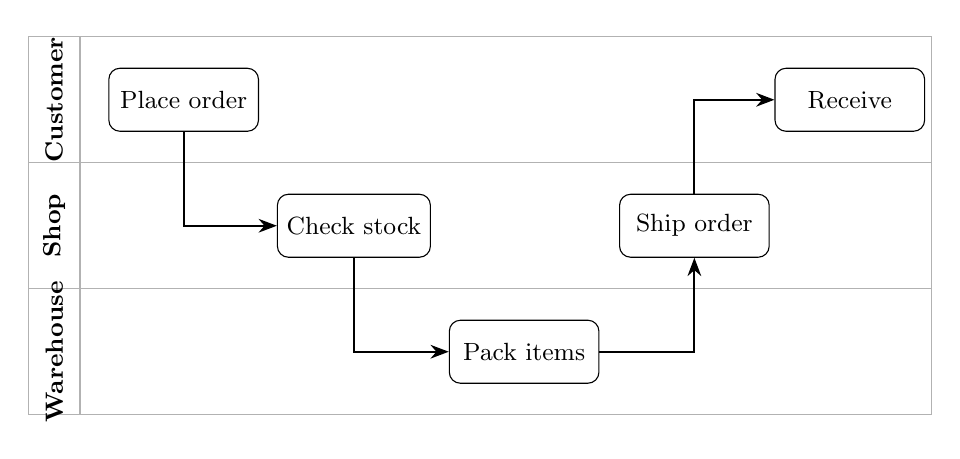
\begin{tikzpicture}[
  x=0.94cm,
  every node/.style={font=\small},
  task/.style={rectangle, rounded corners, draw, minimum width=19mm, minimum height=8mm},
  arrow/.style={-{Stealth}, thick},
]
  \foreach \y/\lane in {0/Customer, -1.6/Shop, -3.2/Warehouse} {
    \draw[gray!60] (0,\y+0.8) rectangle (12.2,\y-0.8);
    \node[rotate=90, font=\small\bfseries] at (0.35,\y) {\lane};
  }
  \draw[gray!60] (0.7,0.8) -- (0.7,-4);

  \node[task] (order) at (2.1,0) {Place order};
  \node[task] (check) at (4.4,-1.6) {Check stock};
  \node[task] (pack) at (6.7,-3.2) {Pack items};
  \node[task] (ship) at (9,-1.6) {Ship order};
  \node[task] (receive) at (11.1,0) {Receive};

  \draw[arrow] (order) |- (check);
  \draw[arrow] (check) |- (pack);
  \draw[arrow] (pack) -| (ship);
  \draw[arrow] (ship) |- (receive);
\end{tikzpicture}
